\documentclass[12pt,a4paper]{article}
\usepackage[utf8]{inputenc}
\usepackage[T1]{fontenc}
%\usepackage[czech]{babel}
\usepackage{a4wide}
\usepackage{amsmath, amsthm, amsfonts, amssymb, graphicx, url, fancyhdr,multicol,enumerate,mathtools,tikz}
\newcommand{\norm}[1]{\left\lVert#1\right\rVert}

\newtheorem{theorem}{Theorem}
\newtheorem{lemma}[theorem]{Lemma}
\newtheorem{cor}[theorem]{Corollary}
\newtheorem{prop}[theorem]{Proposition}

\newcommand{\Cbb}{\mathbb{C}}
\newcommand{\Qbb}{\mathbb{Q}}
\newcommand{\Rbb}{\mathbb{R}}
\newcommand{\Zbb}{\mathbb{Z}}
\newcommand{\Nbb}{\mathbb{N}}
\newcommand{\C}{\mathbb{C}}
\newcommand{\Q}{\mathbb{Q}}
\newcommand{\R}{\mathbb{R}}
\newcommand{\Z}{\mathbb{Z}}
\newcommand{\F}{\mathbb{F}}
%\newcommand{\N}{\mathbb{N}}
\newcommand{\id}{\mathrm{id}}
\newcommand{\im}{\mathrm{im}}
\newcommand{\cok}{\mathrm{coker}}
\newcommand{\Hom}{\mathrm{Hom}}
\newcommand{\Max}{\mathrm{Max}}
\newcommand{\disc}{\mathrm{disc}}
\newcommand{\Gal}{\mathrm{Gal}}
\newcommand{\Tr}{\mathrm{Tr}}
\newcommand{\N}{\mathrm{N}}
\newcommand{\No}{\mathrm{N}_{\Qbb}^K}
\newcommand{\Ok}{\ensuremath{\mathcal{O}_K}}
\newcommand{\Ol}{\ensuremath{\mathcal{O}_L}}
\newcommand{\Cl}{\ensuremath{\mathcal{C}l}}
\newcommand{\p}{\mathfrak{p}}
\newcommand{\qq}{\mathfrak{q}}
\newcommand{\af}{\mathfrak{a}}
\newcommand{\bb}{\mathfrak{b}}
\newcommand{\rr}{\mathfrak{r}}
\newcommand{\al}{\alpha}
\newcommand{\Mat}{\ensuremath{\text{Mat}(2,\mathbb{Z})}}
\newcommand{\Char}{\mathrm{char }}
\newcommand{\lcm}{\mathrm{lcm}}

\newcommand\restr[2]{{% we make the whole thing an ordinary symbol
  \left.\kern-\nulldelimiterspace % automatically resize the bar with \right
  #1 % the function
  %\vphantom{\big|} % pretend it's a little taller at normal size
  \right|_{#2} % this is the delimiter
  }}

\begin{document}
%\pagestyle{fancy}                      %Pro větší­ možnosti práce se záhlaví­mi a zápatími
%\fancyhf{}                             %"vvyčištění záhlaví a zápatí"                                         
%\renewcommand{\headheight}{25 pt}                  %
\addtolength{\topmargin}{-30 pt}                   %
\setlength{\headsep}{10 pt}                      %
%\fancyhead[L]{{\emph{M8195/01 Seminář z teorie čísel, podzim 2016, úkol 1}}}  %
%\fancyhead[R]{{\emph{Vladimír Sedláček, učo 408178}}}                 % Nastavení­ pro titulní­ stranu
%\fancyfoot[L]{Školní rok 2009/2010}                %
%\renewcommand{\footrulewidth}{0.8 pt}              %
\renewcommand{\headrulewidth}{1 pt}                %               %

\title{Circular numbers of certain abelian fields}
\author{Vladimír Sedláček}
\date{\today}
\maketitle

Throughout this thesis, we will use the convention that whenever any of the indices $i,j,l,h$ appear on the same line, they are pairwise distinct and moreover $1\leq i,j,l,h\leq 4$.

\section{Basic definitions and assumptions}
Let $k$ be a real abelian field with exactly four ramified primes $p_1,p_2,p_3,p_4$. Let $K$ be the genus field (in the narrow sense) of $k$ and assume $K\neq k$. Let $G:=\Gal(K/\Q)$, then (by the properties of the genus field) we can make the identification $G=T_1\times T_2\times T_3\times T_4$, where $T_i$ is the inertia group corresponding the ramified prime $p_i$. Next, we will define:

\begin{itemize}
\item $H:=\Gal(K/k)$, 
\item $m:=|H|,$
\item the canonical projections $\pi_i:G\to T_i$ ,
\item $a_i:=[T_i:\pi_i(H)]$,
\item $r_i:=|H\cap \ker \pi_i|$,
\item $s_{ij}:=|H\cap \ker (\pi_i\pi_j)|$,
\item $n_i:=\frac{m}{r_i}$,
\item $K_i$ as the maximal subfield of $K$ ramified only at $p_i$ (so that $$T_i=\Gal(K/K_jK_lK_h)\cong \Gal(K_i/\Q).)$$
\end{itemize}

We will assume the following:
\begin{itemize}
\item $K\neq k$,
\item $H$ is cyclic, generated by $\tau$,
\item each $T_i$ is cyclic, generated by $\sigma_i$.
\end{itemize}

\section{Auxiliary results}

\begin{lemma}\label{comp}
We have $kK_iK_jK_l=K$ and $K_1K_2K_3K_4=K$.
\end{lemma}
\begin{proof}
The extension $K/K_iK_jK_l$ is totally ramified at the prime ideals above $p_h$, so the same must be true for the extension $K/kK_iK_jK_l$. But since the extension $K/k$ is unramified (by the definition of $K$), so is $K/kK_iK_jK_l$. Therefore $[K:kK_iK_jK_l]=1$. The second claim follows from the fact $\Gal(K_i/\Q)=T_i$.
\end{proof}
\begin{center}
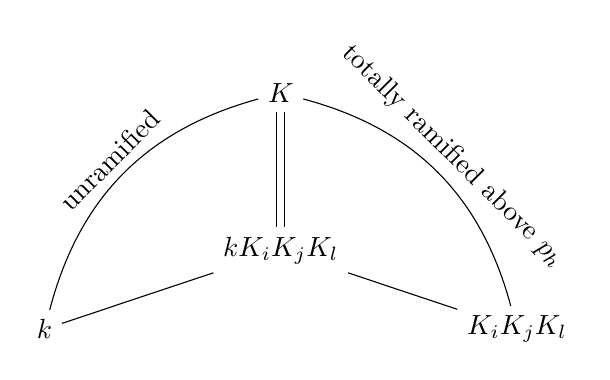
\begin{tikzpicture}
  \node (a) at (0,4)  {$K$};
  \node (b) at (0,2)  {$kK_iK_jK_l$};
  \node (c) at (-3,1)  {$k$};
  \node (d) at (3,1)  {$K_iK_jK_l$};
  \draw[transform canvas={xshift=-1.5pt}] (a) -- (b);
  \draw[transform canvas={xshift=1.5pt}] (b) -- (a);
  \draw   (b) --  (c)
   (b) -- (d);
  \draw[bend left](c) to node [above , sloped]{\text{unramified}}(a);
  \draw[bend right](d) to node [above , sloped]{\text{totally ramified above $p_h$}}(a);
\end{tikzpicture}
\end{center}
%Přidat zvláštní lemma o Galoisových grupách K_iK_jK_l/K_i a podobně kvůli čitelnosti?

\begin{prop}\label{degrees}
We have $a_i=[k\cap K_i:\Q]$, $r_i=[K:kK_i]$, $|T_i|=a_i\frac{m}{r_i}$,  $s_{ij}=[K:kK_iK_j]$. Also $[K_i:k\cap K_i]=\frac{m}{r_i}$, $[K_iK_j:k\cap K_iK_j]=\frac{m}{s_{ij}}$ and $[K_iK_jK_l:k\cap K_iK_jK_l]=m$.
\end{prop}
\begin{proof}
Since
\begin{equation*}
\begin{split}
\Gal(K/K_i)&=\Gal(K/K_iK_jK_l\cap K_iK_jK_h\cap K_iK_lK_h)\\
&=\Gal(K/K_iK_jK_l)\cdot \Gal(K/K_iK_jK_h)\cdot \Gal(K/K_iK_lK_h)
= T_jT_lT_h
\end{split}
\end{equation*} 
%$$\Gal(K/K_i)\cong \Gal(K/\Q)/\Gal(K_i/\Q)\cong T_1T_2T_3T_4/T_i\cong T_jT_lT_h$$
 and $\Gal(K/k)=H$, it follows that $\Gal(K/k\cap K_i)= T_jT_lT_h\cdot H$. Now consider the short exact sequence %(clearly $\ker \pi_i=T_jT_lT_h$) 
$$0\to H\cap \ker \pi_i\to H \xrightarrow{\restr{\pi_i}{H}} \pi_i(H)\to 0.$$
It follows that $|\pi_i(H)|=\frac{m}{r_i}$ and $$\pi_i(H)\cong \frac{H}{H\cap \ker \pi_i}=\frac{H}{H\cap T_jT_lT_h}\cong \frac{T_jT_lT_h\cdot H}{T_jT_lT_h}= \frac{\Gal(K/k\cap K_i)}{\Gal(K/K_i)}\cong \Gal(K_i/k\cap K_i).$$
Therefore 
$$[k\cap K_i:\Q]=\frac{|\Gal(K_i/\Q)|}{|\Gal(K_i/k\cap K_i)|}=\frac{|T_i|}{|\pi_i(H)|}=a_i$$
%$$[k\cap K_i:\Q]=\frac{|T_1T_2T_3T_4|}{|T_jT_lT_h\cdot H|}=\frac{|T_1T_2T_3T_4|\cdot |H\cap T_jT_lT_h|}{|T_jT_lT_h|\cdot |H|}=\frac{|T_i|}{|\pi_i(H)|}=a_i.$$
and
$$[K:kK_i]=\frac{|\Gal(K/k)|}{|\Gal(kK_i/k)|}=\frac{|H|}{|\Gal(K_i/k\cap K_i)|}=\frac{m}{|\pi_i(H)|}=r_i.$$
Putting everything together, we obtain $$|T_i|=[K_i:k\cap K_i]\cdot[k\cap K_i:\Q]=a_i|\pi_i(H)|=a_i\frac{m}{r_i}.$$
Next, we also have 
\begin{equation*}
\begin{split}
\Gal(K/K_iK_j)&=\Gal(K/K_iK_jK_l\cap K_iK_jK_h)\\
&=\Gal(K/K_iK_jK_l)\cdot \Gal(K/K_iK_jK_h)= T_jT_lT_h
\end{split}
\end{equation*} 
%$$\Gal(K/K_iK_j)\cong \Gal(K/\Q)/\Gal(K_iK_j/\Q)\cong T_1T_2T_3T_4/T_iT_j\cong T_lT_h,$$
so that $\Gal(K/k\cap K_iK_j)=T_lT_h\cdot H$. Thus we can consider the short exact sequence 
$$0\to H\cap \ker \pi_i\pi_j\to H \xrightarrow{\restr{\pi_i\pi_j}{H}} \pi_i\pi_j(H)\to 0$$
to conclude that $|\pi_i\pi_j(H)|=\frac{m}{s_{ij}}$ and 
\begin{equation*}
\begin{split}
\pi_i\pi_j(H)&\cong \frac{H}{H\cap \ker \pi_i\pi_j}=\frac{H}{H\cap T_lT_h}\cong \frac{T_lT_h\cdot H}{T_lT_h}\\
&\cong \frac{\Gal(K/k\cap K_iK_j)}{\Gal(K/K_iK_j)}\cong \Gal(K_iK_j/k\cap K_iK_j).
\end{split}
\end{equation*}
Then it follows that 
$$[K:kK_iK_j]=\frac{|\Gal(K/k)|}{|\Gal(kK_iK_j/k)|}=\frac{|H|}{|\Gal(K_iK_j/k\cap K_iK_j)|}=\frac{m}{\pi_i\pi_j(H)}=s_{ij}.$$
The last part of the statement is a consequence of Lemma \ref{comp}, since we have $$\Gal(K_iK_jK_l/k\cap K_iK_jK_l)\cong \Gal(kK_iK_jK_l/k)=\Gal(K/k)=H.$$
Finally note that in the same way as above, we could show that $$\pi_i\pi_j\pi_l(H)\cong \frac{H}{H\cap T_h}\cong H$$
(since Lemma \ref{comp} implies that $|H\cap T_h|=1$).
%Finally note that in the same way as above, we could show that $$\pi_i\pi_j\pi_l(H)\cong \Gal(K_iK_jK_l/k\cap K_iK_jK_l).$$
\end{proof}
\begin{center}
\begin{tikzpicture}
  \node (a) at (0,4)  {$K$};
  \node (b) at (0,2)  {$kK_i$};
  \node (c) at (-2,0)  {$k$};
  \node (d) at (2,0)  {$K_i$};
  \node (e) at (0,-2)  {$k\cap K_i$};
  \node (f) at (0,-4)  {$\Q$};
  \draw   (a) -- node [left]{$r_i$} (b) -- node [above left]{$\frac{m}{r_i}$} (c) -- (e) -- node [below right]{$|\pi_i(H)|$} (d) -- node [above right]{$\frac{|T_j\times T_l\times T_h|}{r_i}$} (b)
  (e) -- node [left]{$a_i$} (f);
\end{tikzpicture}
\qquad
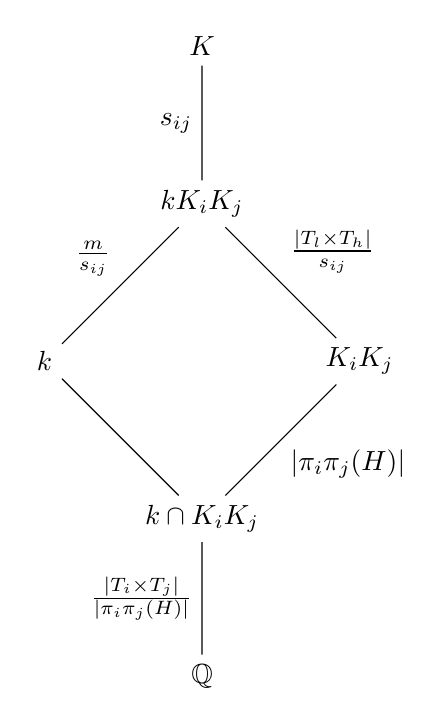
\begin{tikzpicture}
  \node (a) at (0,4)  {$K$};
  \node (b) at (0,2)  {$kK_iK_j$};
  \node (c) at (-2,0)  {$k$};
  \node (d) at (2,0)  {$K_iK_j$};
  \node (e) at (0,-2)  {$k\cap K_iK_j$};
  \node (f) at (0,-4)  {$\Q$};
  \draw   (a) -- node [left]{$s_{ij}$} (b) -- node [above left]{$\frac{m}{s_{ij}}$} (c) -- (e) -- node [below right]{$|\pi_i\pi_j(H)|$} (d) -- node [above right]{$\frac{|T_l\times T_h|}{s_{ij}}$} (b)
  (e) -- node [left]{$\frac{|T_i\times T_j|}{|\pi_i\pi_j(H)|}$} (f);
\end{tikzpicture}
%\vspace{3\baselineskip}
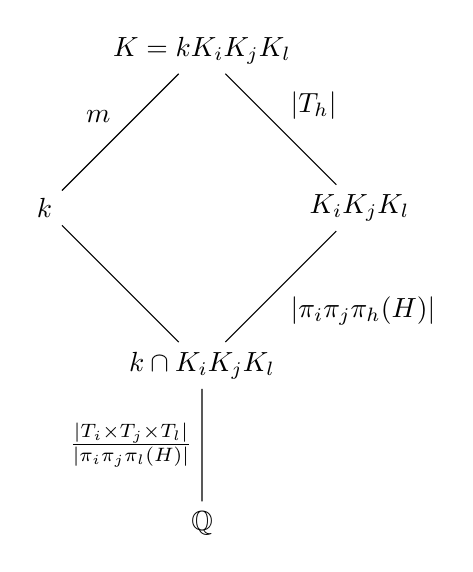
\begin{tikzpicture}
  \node (a) at (0,2)  {$K=kK_iK_jK_l$};
  \node (c) at (-2,0)  {$k$};
  \node (d) at (2,0)  {$K_iK_jK_l$};
  \node (e) at (0,-2)  {$k\cap K_iK_jK_l$};
  \node (f) at (0,-4)  {$\Q$};
  \draw   (a) -- node [above left]{$m$} (c) -- (e) -- node [below right ]{$|\pi_i\pi_j\pi_h(H)|$} (d) -- node [above right]{$|T_h|$} (a)
  (e) -- node [left]{$\frac{|T_i\times T_j\times T_l|}{|\pi_i\pi_j\pi_l(H)|}$} (f);
\end{tikzpicture}
\end{center}

\begin{cor}\label{compcap}
We have $[k\cap K_iK_j:\Q]=a_ia_j\frac{m}{r_ir_j}s_{ij}$, $[k\cap K_iK_jK_l:\Q]=a_ia_ja_l\frac{m^2}{r_ir_jr_l}$ and $[k:\Q]=a_1a_2a_3a_4\frac{m^3}{r_1r_2r_3r_4}$.
\end{cor}
\begin{proof}
This follows from the computations
$$[k\cap K_iK_j:\Q]=\frac{[K_iK_j:\Q]}{[K_iK_j:k\cap K_iK_j]}=\frac{|T_i|\cdot|T_j|}{m/s_{ij}}=a_ia_j\frac{m}{r_ir_j}s_{ij},$$
$$[k\cap K_iK_jK_l:\Q]=\frac{[K_iK_jK_l:\Q]}{[K_iK_jK_l:k\cap K_iK_jK_l]}=\frac{|T_i|\cdot|T_j|\cdot|T_l|}{m}=a_ia_ja_l\frac{m^2}{r_ir_jr_l}$$
and
\begin{equation*}
\begin{split}
[k:\Q]&=[k\cap K_i:\Q]\cdot [k:k\cap K_i]=a_i\cdot [kK_i:K_i]=a_i\frac{[K:K_i]}{[K:kK_i]}\\
&=a_i\frac{|T_j|\cdot|T_l|\cdot|T_h|}{r_i}=
a_1a_2a_3a_4\frac{m^3}{r_1r_2r_3r_4}.
\end{split}
\end{equation*}

\end{proof}
\begin{lemma}\label{coprime}
We have $s_{ij}=\gcd(r_i,r_j)$, $\gcd(r_i,r_j,r_l)=1$ (this is also equivalent to $\lcm\left(\frac{m}{r_i},\frac{m}{r_j},\frac{m}{r_l}\right)=m$ and to $\gcd(s_{ij},r_l)=1$) and $s_{ij}\frac{m}{r_ir_j}=\gcd(\frac{m}{r_i},\frac{m}{r_j})$.
\end{lemma}
\begin{proof}
It follows from Proposition \ref{degrees} that $s_{ij}\mid r_i, s_{ij}\mid r_j$ and from its proof that $|\pi_i(H)|=\frac{m}{r_i}$, $|\pi_i\pi_j(H)|=\frac{m}{s_{ij}}$ and $|\pi_i\pi_j\pi_l(H)|=m$. The cyclicity of $H$ then implies
$$\frac{m}{s_{ij}}=|\pi_i\pi_j(H)|=|\langle\pi_i\pi_j(\tau)\rangle|=|\langle\pi_i(\tau)\pi_j(\tau)\rangle|=\lcm\left(\frac{m}{r_i},\frac{m}{r_j}\right),$$
because $\langle\pi_i(\tau)\rangle=\pi_i(H)$ and any power of the product $\pi_i(\tau)\pi_j(\tau)$ is trivial if and only if the same power of both its factors is (since $G$ is the direct product of the $T_i$'s). 
%the elements $\pi_i(H),\pi_j(H)$ have different non-zero coordinates in $G$.
Now for any common divisor $t$ of $r_i,r_j$, we have $\frac{m}{s_{ij}}= \lcm\left(\frac{m}{r_i},\frac{m}{r_j}\right) \mid \frac{m}{t}$, which implies $t\mid s_{ij}$ and we are done.

Similarly, we have
$$m=|\pi_i\pi_j\pi_l(H)|=|\langle\pi_i\pi_j\pi_l(\tau)\rangle|=|\langle\pi_i(\tau)\pi_j(\tau)\pi_l(\tau)\rangle|=\lcm\left(\frac{m}{r_i},\frac{m}{r_j},\frac{m}{r_l}\right),$$
so if $t$ is any common divisor of $r_i,r_j,r_l$, we have $m=\lcm\left(\frac{m}{r_i},\frac{m}{r_j},\frac{m}{r_l}\right)\mid \frac{m}{t}$, which implies $t=1$.

Finally, using the first result, we have $s_{ij}\frac{m}{r_ir_j}=\frac{m}{\lcm(r_i,r_j)}$, which clearly divides both $\frac{m}{r_i}$ and $\frac{m}{r_j}$. Moreover, if $t$ is any common divisor of $\frac{m}{r_i}$ and $\frac{m}{r_j}$, then both $r_it$ and $r_jt$ divide $m$, hence $t\cdot\lcm(r_i,r_j)=\lcm(r_it,r_jt)\mid m$. Thus $t\mid \frac{m}{\lcm(r_i,r_j)}$ and we are done.
\end{proof}

\begin{prop}\label{gal}
We have 
\begin{equation*}
\begin{split}
\Gal(k/\Qbb)\cong
 \{\restr{\left(\sigma_1^{x_1}\sigma_2^{x_2}\sigma_3^{x_3}\sigma_4^{x_4}\right)}{k};~ & 0\leq x_1<a_1\frac{m}{r_1}, 0\leq x_2<a_2\frac{m}{r_2s_{34}}, \\ & 0\leq x_3<a_3\frac{m}{r_3r_4}s_{34},0\leq x_4<a_4\},
\end{split}
\end{equation*}
where each automorphism of $k$ determines the quadruple $(x_1,x_2,x_3,x_4)$ uniquely.
\end{prop}
\begin{proof}
First off, the cardinalities of the sets on both sides agree. Now let $\rho$ be any automorphism of $k$. Since $\Gal(k\cap K_4/\Q)$ is a cyclic group of order $a_4$ (by lemma \ref{degrees}) generated by $\restr{\sigma_4}{k\cap K_4}$ (as a quotient of $\Gal(K_4/\Q)=\langle \restr{\sigma_4}{K_4}\rangle$), there must exist a unique $x_4\in \Z$, $0\leq x_4<a_4$ such that $\rho$ and $\sigma_4^{x_4}$ have the same restrictions to $k\cap K_4$. Therefore $\rho\restr{\sigma_4^{-x_4}}{k}\in \Gal(k/k\cap K_4)$. 

Next, $\Gal(k\cap K_3K_4/k\cap K_4)$ is a cyclic group of order $\frac{[k\cap K_3K_4:\Q]}{[k\cap K_4:\Q]}=a_3\frac{m}{r_3r_4}s_{34}$ (by Corollary \ref{compcap}) generated by $\restr{\sigma_3}{k\cap K_3K_4}$ (as a quotient of $\Gal(K_3K_4/K_4)=\langle \restr{\sigma_3}{K_3K_4}\rangle$), so there must exist a unique $x_3\in \Z$, $0\leq x_3<a_3\frac{m}{r_3r_4}s_{34}$ such that $\rho\sigma_4^{-x_4}$ and $\sigma_3^{x_3}$ have the same restriction to $k\cap K_3K_4$. Therefore $\restr{\rho\sigma_3^{-x_3}\sigma_4^{-x_4}}{k}\in \Gal(k/k\cap K_3K_4)$.

Following the pattern, $\Gal(k\cap K_2K_3K_4/k\cap K_3K_4)$ is a cyclic group of order 
$$\frac{[k\cap K_2K_3K_4:\Q]}{[k\cap K_3K_4:\Q]}=a_2\frac{m}{r_2s_{34}}$$ (by Corollary \ref{compcap}) generated by $\restr{\sigma_2}{k\cap K_2K_3K_4}$ (as a quotient of $$\Gal(K_2K_3K_4/K_3K_4)=\langle \restr{\sigma_2}{K_2K_3K_4}\rangle),$$ so there must exist a unique $x_2\in \Z$, $0\leq x_2<a_2\frac{m}{r_2s_{34}}$ such that $\rho\sigma_3^{-x_3}\sigma_4^{-x_4}$ and $\sigma_2^{x_2}$ have the same restriction to $k\cap K_2K_3K_4$. Therefore $\restr{\rho\sigma_2^{-x_2}\sigma_3^{-x_3}\sigma_4^{-x_4}}{k}\in \Gal(k/k\cap K_2K_3K_4)$.

Finally, we have $$\Gal(k/k\cap K_2K_3K_4)\cong \Gal(kK_2K_3K_4/K_2K_3K_4)=\Gal(K_1K_2K_3K_4/K_2K_3K_4)=\langle\sigma_1\rangle$$
(using Lemma \ref{comp}), where the isomorphism is given by restriction. Since the order of $\sigma_1$ is $a_1\frac{m}{r_1}$, it follows that there must exist a unique $x_1\in \Z$, $0\leq x_1<a_1\frac{m}{r_1}$ such that $\rho\sigma_2^{-x_2}\sigma_3^{-x_3}\sigma_4^{-x_4}$ and $\sigma_1^{x_1}$ have the same restriction to $k$. Thus $\rho=\sigma_1^{x_1}\sigma_2^{x_2}\sigma_3^{x_3}\sigma_4^{x_4}$ and the proof is finished.
\begin{center}
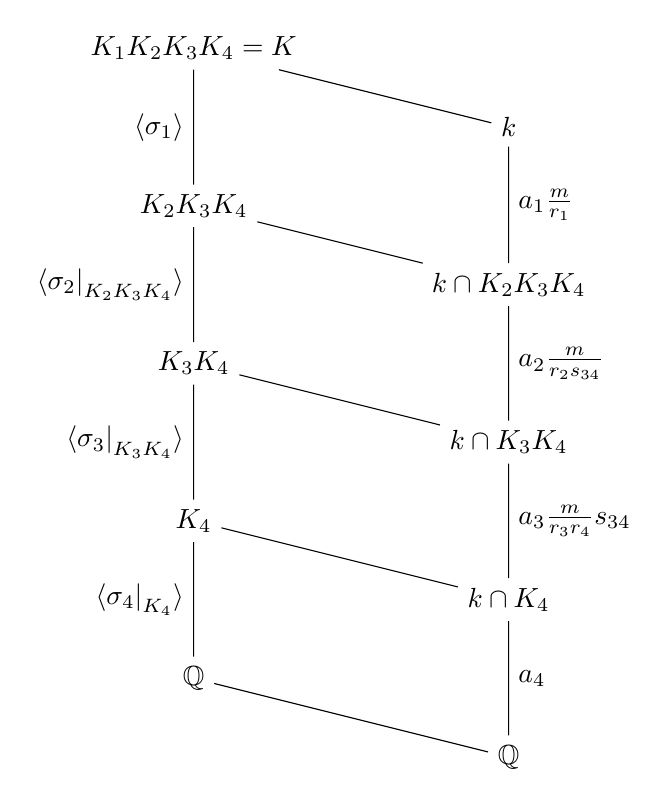
\begin{tikzpicture}
  \node (a) at (0,4)  {$K_1K_2K_3K_4=K$};
  \node (b) at (4,3)  {$k$};
  \node (c) at (0,2)  {$K_2K_3K_4$};
  \node (d) at (4,1)  {$k\cap K_2K_3K_4$};
  \node (e) at (0,0)  {$K_3K_4$};
  \node (f) at (4,-1)  {$k\cap K_3K_4$};
  \node (g) at (0,-2) {$K_4$};
  \node (h) at (4,-3)  {$k\cap K_4$};
  \node (i) at (0,-4) {$\Q$};
  \node (j) at (4,-5)  {$\Q$};
  \draw  (a) -- node [midway,left]{$\langle \sigma_1\rangle$} (c) -- node [midway,left]{$\langle \restr{\sigma_2}{K_2K_3K_4}\rangle$} (e) -- node [midway,left]{$\langle \restr{\sigma_3}{K_3K_4}\rangle$} (g) -- node [midway,left]{$\langle \restr{\sigma_4}{K_4}\rangle$} (i) -- (j) -- node [midway,right]{$a_4$} (h) -- node [midway,right]{$a_3\frac{m}{r_3r_4}s_{34}$} (f) -- node [midway,right]{$a_2\frac{m}{r_2s_{34}}$} (d) -- node [midway,right]{$a_1\frac{m}{r_1}$} (b) -- (a) 
  (c) -- (d)
  (e) -- (f)
  (g) -- (h);
\end{tikzpicture}
\end{center}
\end{proof}

\begin{lemma}
Without loss of generality, we can assume $\tau=\sigma_1^{a_1}\sigma_2^{a_2}\sigma_3^{a_3}\sigma_4^{a_4}$.
\end{lemma}
\begin{proof}
We know that $a_i=[T_i:\pi_i(H)]$, hence
$\pi_i(\tau)$ generates a subgroup of $T_i$ of index $a_i$. The cyclicity of $T_i$ then implies that $\pi_i(\tau)$ must be the $a_i$-th power of some generater of $T_i$, WLOG $\sigma_i$. The statement now follows, because $\tau$ is determined by its four projections.
\end{proof}

\section{The group of circular numbers}

Recall that $D^+$, the subgroup of totally positive elements of the group $D$ of circular numbers of a real abelian field $k'$ (using Lettl's modification of Sinnott's definition), has one generator $\eta_I$ for each nonempty subset $I\subseteq P$, where $P$ is the set of ramified primes of $k'$. (Since $k'$ is real, $D^+$ is also canonically isomorphic to the non-torsion part of $D$.) 

More explicitly, if we let $K'_i$ be the largest subfield of $K'$ (the genus field of $k'$) in which $p_i$ is the only ramified prime for any $i\in I$, we have
$$\eta_I=\text{N}_{\Qbb(\zeta_{\text{cond} \left(\prod_{i\in I}K'_i\right)})/\left(\prod_{i\in I}K'_i)\right)\cap k'}\left(1-\zeta_{\text{cond} \left(\prod_{i\in I}K'_i\right)}\right).$$
It is well known that $D^+$ is a $\Zbb[G]$-module of $\Zbb$-rank $[k:\Qbb]+|P|-1$. 

(In our case, we have $k'=k, K'=K, K'_i=K_i, |P|=4$, $\eta:=\eta_{\{1,2,3,4\}}$.)

%The generators of $D^+$ are subject to norm relations (which can be obtained by computing the norm of the generators to a subfield with less ramified primes) and for $|P|\geq 3$, also to the so-called Ennola relations, which are highly nontrivial relations that are not consequences of the norm relations.

%Our goal will be to find a basis of $D^+$ (it can then be easily modified in order to obtain a basis of the group of circular units). Such a basis is known only in a few very special cases though. We would like to construct it for general abelian fields as well, based only on the number of ramified primes.
\paragraph*{}
Our goal will be to find a basis of $D^+$ (it can then be easily modified in order to obtain a basis of the group of circular units). The generators of $D^+$ are subject to norm relations that correspond to the sum of all elements of the respective inertia groups.

Let $$R_i=\sum_{u=0}^{a_i-1}\sigma_i^u,\, N_i=\sum_{u=0}^{\frac{m}{r_i}-1}\sigma_i^{au_i}.$$ 

Then the norm operators from $k$ to the maximal subfield ramified at less primes can be given as $R_iN_i$ (i.e. the sum of all elements of $T_i$). If we denote the congruence corresponding to the canonical projection $\Z[G]\to \Z[G/H]$ by $\equiv$, then we have $N_4\equiv \sum_{u=0}^{m-1}\sigma_1^{ua_1}\sigma_2^{ua_2}\sigma_3^{ua_3}$.

Moreover, we will denote the congruence corresponding to the composition of canonical projections $\Z[G]\to \Z[G/H]\to \Z[G/H]/(R_1N_1,R_2N_2,R_3N_3,R_4N_4)$ by $\sim$, where $(R_1N_1,R_2N_2,R_3N_3,R_4N_4)$ is the ideal generated in $\Z[G/H]$ by the images of the elements $R_iN_i$. When we apply any element of this ideal to the highest generator $\eta$, we will obtain a circular unit belonging to a field with less ramified primes. We will make use of this extensively.

To construct a basis of $D^+$, we can take the union of all bases for the fields $$k\cap K_1K_2K_3,k\cap K_1K_2K_4,k\cap K_1K_3K_4,k\cap K_2K_3K_4$$ (which have three ramified primes, so we can use the results in [1]) and add in
\begin{equation*}
\begin{split}
c:&=[k:\Q]+3-\sum_{i,j,l}([k\cap K_iK_jK_l:\Q]+2)+\sum_{i,j}([k\cap K_iK_j:\Q]+1)-\sum_{i}[k\cap K_i:\Q]\\&=a_1a_2a_3a_4\frac{m^3}{r_1r_2r_3r_4}-\sum_{i,j,l}a_ia_ja_l\frac{m^2}{r_ir_jr_l}+\sum_{i,j}
a_ia_js_{ij}\frac{m}{r_ir_j}-\sum_{i}a_i+1
\end{split}
\end{equation*}
(by the principle of inclusion and exclusion) conjugates of $\eta$. Then we will need to show how to obtain the missing conjugates of $\eta$ using the relations $$R_1N_1\sim 0, R_2N_2\sim 0, R_3N_3\sim 0, R_4\sum_{u=0}^{m-1}\sigma_1^{ua_1}\sigma_2^{ua_2}\sigma_3^{ua_3}\sim 0.$$

We will always refer to the conjugates of $\eta$ by their coordinates $x_1,x_2,x_3,x_4$ according to Proposition \ref{gal}. This allows for geometric interpretation.

\section{The case $r_1=r_2=a_3=r_4=1$}
(Note that in this case we have $s_{34}=1$.) %, therefore $$c=a_1a_2a_4\frac{m^3}{r_3}-\sum_{i,j,l}a_ia_ja_l\frac{m^2}{r_ir_jr_l}+\sum_{i,j}+a_ia_js_{ij}\frac{m}{r_ir_j}-\sum_{i}a_i+1.$$
\paragraph*{}
We will add all the conjugates of $\eta$ to our basis except the following cases:
\begin{itemize}
\item $x_1=a_1m-1$ or $x_2=a_2m-1$ or $x_3=\frac{m}{r_3}-1$,
\item $a_1\leq x_1 < a_1m-1, a_2(m-1)-1 \leq x_2 < a_2m-1, 0\leq x_3 < \frac{m}{r_3}-1, x_4=0$,
\item $0\leq x_1 < a_1, a_2(m-1) \leq x_2 < a_2m-1, 0\leq x_3 < \frac{m}{r_3}-1, x_4=0$.
\end{itemize}
These cases are all disjoint, so it's easy to see that the number of conjugaters of $\eta$ that we chose is exactly
$$((a_1m-1)a_2(m-2)+(a_1m-1)(a_2-1)+a_1+(a_4-1)(a_1m-1)(a_2m-1))\left(\frac{m}{r_3}-1\right)=c.$$
\paragraph*{}
First we will recover the cases $0<x_4<a_4$, $x_1=a_1m-1$ or $x_2=a_2m-1$ or $x_3=\frac{m}{r_3}-1$ using the relations $R_1N_1\sim 0, R_2N_2\sim 0, R_3N_3\sim 0$. From now on, we only need to deal with the cases where $x_4=0$.
\paragraph*{}
Next, we will recover the cases $$x_1=a_1m-1, 0\leq x_2 < a_2(m-1)-1, 0\leq x_3 <\frac{m}{r_3}-1$$ using the relation $R_1N_1\sim 0$ and subsequently the cases $$0\leq x_1 < a_1m-1, 0\leq x_2 < a_2(m-1)-1, 0\leq x_3 <\frac{m}{r_3}-1$$ and $$0\leq x_1 < a_1-1, x_2 = a_2(m-1)-1, 0\leq x_3 <\frac{m}{r_3}-1$$ using the relation $R_3N_3\sim 0$.
\paragraph*{}
Next, we will sequentially recover all the cases $$0\leq x_1 < a_1m-1, a_2(m-1)\leq x_2 < a_2m-1, 0\leq x_3 <\frac{m}{r_3}-1$$
using the relation $R_4\sum_{u=0}^{m-1}\sigma_1^{a_1u}\sigma_2^{a_2u}\sigma_3^u$. We can do this since any two conjugates of $\eta$ used in this relation differ by at least $a_2$ in their second coordinate. After this, we can recover the cases $$0\leq x_1 < a_1, x_2 = a_2m-1, 0\leq x_3 <\frac{m}{r_3}-1$$ using the relation $R_2N_2\sim 0$.
\paragraph*{}
Finally, we can use the relation $R_4\sum_{u=0}^{m-1}\sigma_1^{a_1u}\sigma_2^{a_2u}\sigma_3^u$ to recover the cases $$a_1 \leq x_1 <2a_1, x_2 =a_2m-1, 0\leq x_3 <\frac{m}{r_3}-1$$ and subsequently $R_4\sum_{u=0}^{m-1}\sigma_1^{a_1u}\sigma_2^{a_2u}\sigma_3^u$ to recover the cases $$a_1 \leq x_1 <2a_1, x_2 =a_2(m-1)-1, 0\leq x_3 <\frac{m}{r_3}-1.$$ By repeating these two steps $(m-2)$ more times, increasing the first coordinate by $a_1$ each time, we will recover all the conjugates.

\section{The case $a_1=a_2=r_3=r_4=1$}
(Recall that $n_i=\frac{m}{r_i}$.)

In this case, using Lemma \ref{coprime}, we have
\begin{equation*}
\begin{split}
c&=a_3\left(n_1-1\right)\left(n_2-1\right)\left(m-1\right)-\left(n_1-1\right)\left(n_2-1\right)+\gcd\left(n_1,n_2\right)-1\\
&+(a_4-1)\left(a_3\left(n_1-1\right)\left(n_2-1\right)m-\left(n_1-1\right)\left(n_2-1\right)\right).
\end{split}
\end{equation*}
We will add the following $c$ conjugates of $\eta$ to our basis:
\begin{itemize}
\item $0\leq x_1<n_1-1, 0\leq x_2<n_2-1, 0\leq x_3<a_3m-1, 0<x_4\leq a_4-1$,
\item $0\leq x_1<n_1-1, 0\leq x_2<n_2-1, 0\leq x_3<a_3(m-1)-1, x_4=0$,
\item $n_1-(\gcd\left(n_1,n_2\right)-1)\leq x_1\leq n_1-1, x_2=n_2-1, x_3=a_3m-1, x_4=0$.
\end{itemize}

\paragraph*{}
First we will recover the cases $0<x_4<a_4$, $x_1=n_1-1$ or $x_2=n_2-1$ or $x_3=a_3m-1$ using the relations $N_1\sim 0, N_2\sim 0, R_3N_3\sim 0$. From now on, we only need to deal with the cases where $x_4=0$.
\paragraph*{}
Next, we will recover the cases $0\leq x_3<a_3(m-1)-1$, $x_1=n_1-1$ or $x_2=n_2-1$ using the relations $N_1\sim 0, N_2\sim 0$. Now we can also use the relation $R_4\sum_{u=0}^{m-1}\sigma_1^{u}\sigma_2^{u}\sigma_3^{a_3u}\sim 0$ multiple times to recover the cases $$0\leq x_1\leq n_1-1, 0\leq x_2\leq n_2-1, a_3(m-1)\leq x_3<a_3m-1.$$
\paragraph*{}
At this moment, we are only missing all the cases with $x_3=a_3(m-1)-1$ and some of those with $x_3=a_3m-1$. 
Let's focus on the second kind. The conjugates with $x_3=a_3m-1$ (and $x_4=0$) can be visualized as a discrete rectangle with sides $n_1$ and $n_2$. It is easy to see that such a rectangle can be partitioned into $\gcd(n_1,n_2)$ diagonals, each containing $\lcm(n_1,n_2)$ elements (two conjugates lie in the same diagonal iff one can be obtained from the other as a multiple of $\sigma_1^v\sigma_2^v$ for some $v\in\Z$). Now consider the relations $$T:=-\left(\sigma_3^{a_3-1}R_4\sum_{u=0}^{m-1}\sigma_1^{u}\sigma_2^{u}\sigma_3^{a_3u}\right)-\sigma_1^{\frac{m}{r_1}-2}\sigma_2^{\frac{m}{r_2}-2} R_3N_3$$
and
$$S_v:=\sum_{u=0}^{v}\sigma_1^{-u}\sigma_2^{-u}T \text{ for } v\in\Z.$$
Clearly $T\sim 0, S_v\sim 0$ for all $v\in\Z$. Also note that for any $v$, $S_v$ contains no conjugate with $x_3=a_3(m-1)-1$ and contains exactly one conjugate with $x_3=a_3m-1$ that we cannot recover yet minus $\sigma_3^{a_3m-1}$, and these two always lie on the same diagonal. Moreover, any conjugate sharing this diagonal can occur as the one with positive sign for suitable $v\in\Z$. Therefore, since we already have the conjugates $$n_1-(\gcd\left(n_1,n_2\right)-1)\leq x_1\leq n_1-1, \leq x_2=n_2-1, x_3=a_3m-1$$ in our basis, we can recover all the conjugates that share the same diagonal with any (and therefore all) of these.
\paragraph*{}
Now we can recover all the conjugates with $x_3=a_3m-1$ except $\lcm(n_1,n_2)$ of them, which share a diagonal. By using the relation $\sigma_1^{\gcd\left(n_1,n_2\right)-1}\left(S_v-S_w\right)\sim 0$ for suitable $v,w\in\Z$, it is clear that we can generate the difference of any two conjugates lying on this diagonal. Now let $$n_1':=\frac{n_1}{\gcd\left(n_1,n_2\right)}, \quad n_2':=\frac{n_2}{\gcd\left(n_1,n_2\right)}$$ and
note that in each column, there are exactly $n_1'$ conjugates lying on this diagonal, and in each row, there are exactly $n_2'$ conjugates lying on this diagonal. Moreover, we have $$\gcd\left(n_1',n_2'\right)=1$$ by construction,
so there exists an integer $z>0$ such that $$n_2'z\equiv 1\pmod{n_1'}.$$
Using the observation above, we can generate $n_2'z$ differences of conjugates lying on the last diagonal in such a way that we will obtain each of the conjugates in the row $x_1=0$ exactly $z$ times with a negative sign, each of the conjugates in the column $x_2=0$ exactly $\frac{n_2'z-1}{n_1'}$ times with a positive sign and finally one conjugate with a positive sign with $$x_1=n_1-(\gcd\left(n_1,n_2\right)-1)-1,x_2=n_2-1.$$
 %$\frac{\frac{m}{r_2}}{\gcd\left(\frac{m}{r_1},\frac{m}{r_2}\right)}$ conjugates with a negative sign evenly distributed among the row $x_1=0$,  $\frac{\frac{\frac{m}{r_2}}{\gcd\left(\frac{m}{r_1},\frac{m}{r_2}\right)}z-1}{\frac{\frac{m}{r_1}}{\gcd\left(\frac{m}{r_1},\frac{m}{r_2}\right)}}$ conjugates with a positive sign evenly distributed among the column $x_2=0$ and finally one conjugate with a positive sign with $$x_1=a_1\frac{m}{r_1}-(\gcd\left(\frac{m}{r_1},\frac{m}{r_2}\right)-1)-1,x_2=\frac{m}{r_2}-1.$$
We can keep this last one and get rid of the rest using the relations $N_1\sim 0$, $N_2\sim 0$. Using this last one, we can generate the rest of its diagonal in the same way as above. Hence we have recovered all the conjugates with $x_3=a_3m-1$. Finally, using the relation $R_3N_3\sim 0$, we can now recover all the conjugates with $x_3=a_3(m-1)-1$ and we are done.

%$$0\sim\left(\left(\sum_{u=0}^{m-1}\sigma_1^{ua_1}\sigma_2^{ua_2}\sigma_3^{ua_3}\right)+\sigma_1^{\frac{m}{r_1}-2}\sigma_2^{\frac{m}{r_2}-2}N_3\right)\left(\sum_{u=0}^{\frac{\frac{m}{r_1}-3}{2}}\sigma_1^{2u}\right)$$
\section{The module of relations}
\section{Construction of suitable abelian fields}
Let $m,a_1,a_2,a_3,a_4,r_1,r_2,r_3,r_4$ be positive integers such that 
$$m>1, r_i\mid m, \gcd(r_i,r_j,r_l)=1.$$
We will construct an infinite family of fields $k$ that satisfy all of our assumptions such that these integers correspond to the parameters in our problem of the same name.

First, we will fix distinct primes $p_1,p_2,p_3,p_4$ such that $p_i\equiv 1\pmod{ 2a_i\frac{m}{r_i}}$ (by Dirichlet's theorem on primes in arithmetic progressions, there are infinitely many ways of doing this). Then there exist even Dirichlet characters $\chi_i$ of conductors $p_i$ and orders $a_i\frac{m}{r_i}$ (namely, these can be given as $\chi_i:=\chi^{\frac{p_i-1}{a_im_i/r_i}}$, where $\chi$ is any generator of the cyclic group $\widehat{(\Z/p_i\Z)^\times}$ (note that $p_i>2$)).

Now let $K_i$ be the field associated to $\langle \chi_i\rangle$. Then $K_i$ is real (because $\chi_i$ is even) and $\Gal(K_i/\Q)$ is cyclic of order $a_i\frac{m}{r_i}$, say $\Gal(K_i/\Q)=\langle \sigma_i\rangle$. Moreover, since the conductors $p_i$ are coprime, the group $\langle \chi_1,\chi_2,\chi_3,\chi_4\rangle$ corresponds to the compositum field $K=K_1K_2K_3K_4$. By the theory of Dirichlet characters, $K$ is ramified exactly at primes $p_i$ (with inertia subgroups isomorphic to $\Gal(K_i/\Q)$) and $$\Gal(K/\Q)=\Gal(K_1/\Q)\Gal(K_2/\Q)\Gal(K_3/\Q)\Gal(K_4/\Q)=\langle\sigma_1,\sigma_2,\sigma_3,\sigma_4\rangle,$$
so that $[K:\Q]=a_1a_2a_3a_4\frac{m^4}{r_1r_2r_3r_4}$. Now let $\tau:=\sigma_1^{a_1}\sigma_2^{a_2}\sigma_3^{a_3}\sigma_4^{a_4}$ and let $k$ be the subfield of $K$ fixed by $\tau$. Since $k$ is a subfield of a compositum of real fields, it must also be real. In order to reach our goal, we now only need to prove the following theorem (it is not hard to see that we could have used the results from Lemma \ref{comp} and Proposition \ref{degrees} as definitions instead).

\begin{theorem}
In the above notation, we have $[K:k]=m$, $[K:kK_i]=r_i$, $[k\cap K_i:\Q]=a_i$ and $kK_iK_jK_l=K$ (i.e. $K$ is the genus field of $k$).
\end{theorem}
\begin{proof}
Using Lemma \ref{coprime} several times, we can compute
$$[K:k]=|\langle\tau\rangle|=\lcm\left(\frac{m}{r_i},\frac{m}{r_j},\frac{m}{r_l}\right)=m,$$
$$[K:kK_i]=|\langle\tau\rangle\cap \langle\sigma_j\sigma_l\sigma_h\rangle|=|\langle\tau^{a_im/r_i}\rangle|=r_i,$$
$$[k\cap K_i:/\Q]=[\langle\sigma_1,\sigma_2,\sigma_3,\sigma_4\rangle:\langle\tau,\sigma_j,\sigma_l,\sigma_h\rangle]=[\langle\sigma_1,\sigma_2,\sigma_3,\sigma_4\rangle:\langle\sigma_i^{a_i},\sigma_j,\sigma_l,\sigma_h\rangle]=a_i$$
and
$$[K:kK_iK_jK_l]=|\langle\tau\rangle\cap \langle\sigma_h\rangle|=|\langle\tau^{\lcm\left(\frac{m}{r_i},\frac{m}{r_j},\frac{m}{r_l}\right)}\rangle|=|\langle\tau^m\rangle|=1.$$
\end{proof}
\end{document}